\documentclass[9pt]{beamer}
\input{../flat-blue-theme.inc}

\usepackage[utf8]{inputenc}
\usepackage[OT1]{fontenc}
\usepackage[ngerman]{babel}
\usepackage{lastpage}
\usepackage{xcolor}
\usepackage{fontawesome}
\usepackage{lmodern}
\usepackage{tikz}
\usepackage{tabularx}
\usepackage{fancyvrb}

\setbeamercovered{invisible}

\author[Hauke Stieler]{
	Hauke Stieler\n
	\href{https://github.com/hauke96}{\footnotesize\textcolor{gray}{\faicon{github} hauke96}}
}
\title{wiki2book}
\subtitle{Aus Wikipedia eigene Bücher bauen}
\date{\today}

\begin{document}
	{
		\setbeamertemplate{headline}{}
%		\setbeamertemplate{background}{\includegraphics[width=\paperwidth,trim=0 0 0 3.5cm]{images/title}}
		\maketitle
	}

	% Kurze Infos zu mir?

	% Motivation
	% - Abstieg in immer tiefere Wikipedia Artikel
	% - Warum nicht tool XY?
	\section{Motivation}	
	
	\subsection{Wikipedia hole}
	
	\begin{frame}
		\begin{center}
			Kennt ihr das?
		\end{center}
	\end{frame}

	\begin{frame}
		\begin{center}
			\begin{tikzpicture}
				\visible<1->{\node at (0,0)			{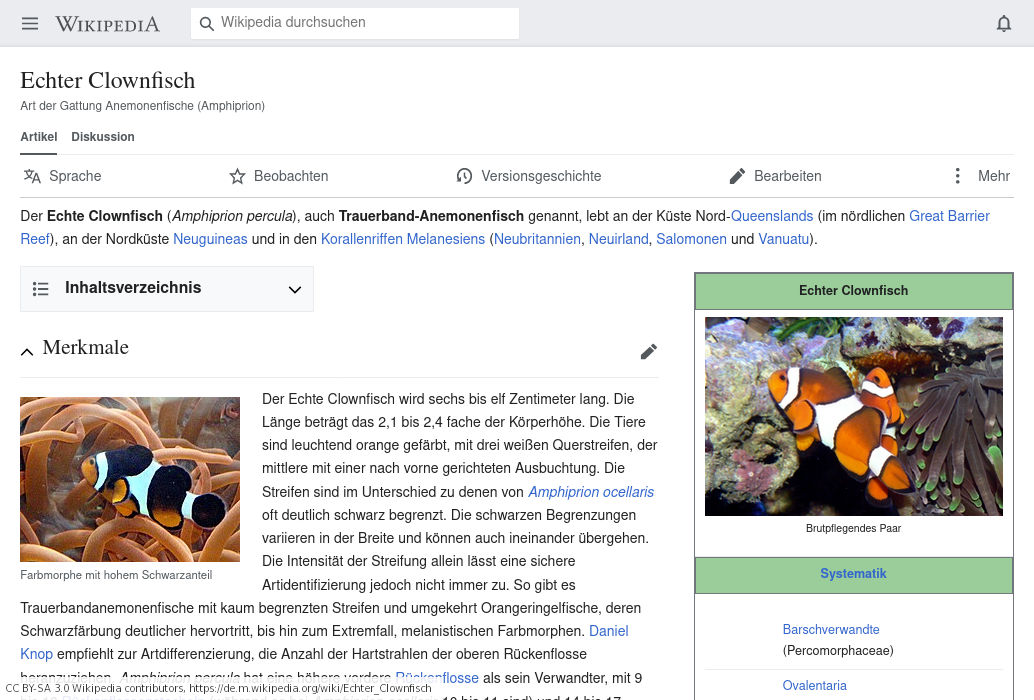
\includegraphics[height=0.75\textheight]{images/wikipedia-screenshot-0.jpg}};}
				\visible<2->{\node at (0.25, -0.25)	{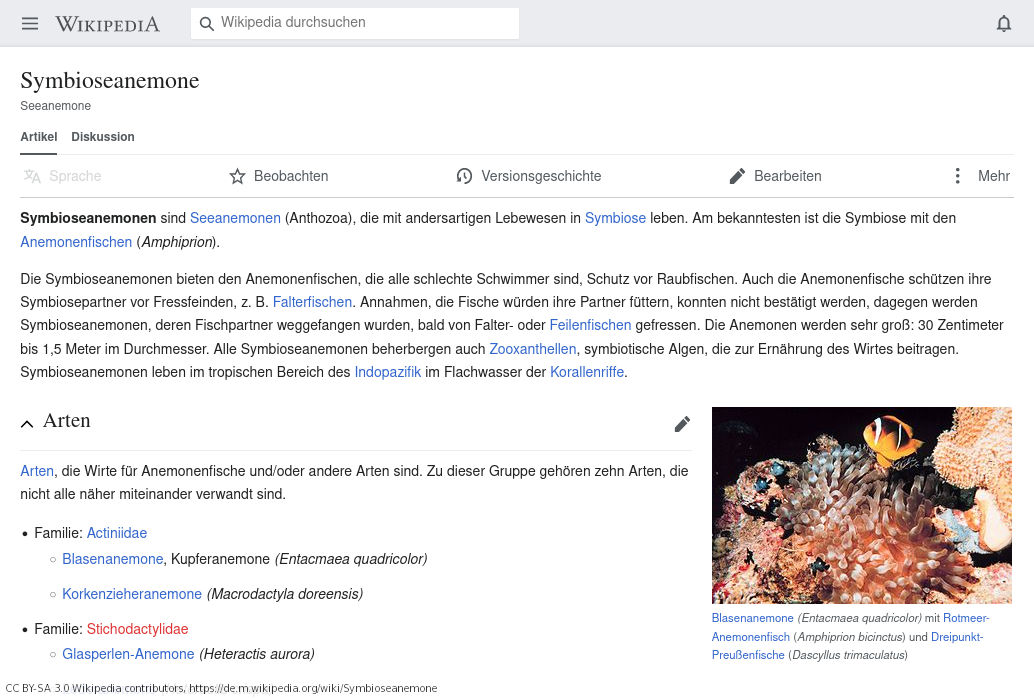
\includegraphics[height=0.75\textheight]{images/wikipedia-screenshot-1.jpg}};}
				\visible<3->{\node at (0.5, -0.5)	{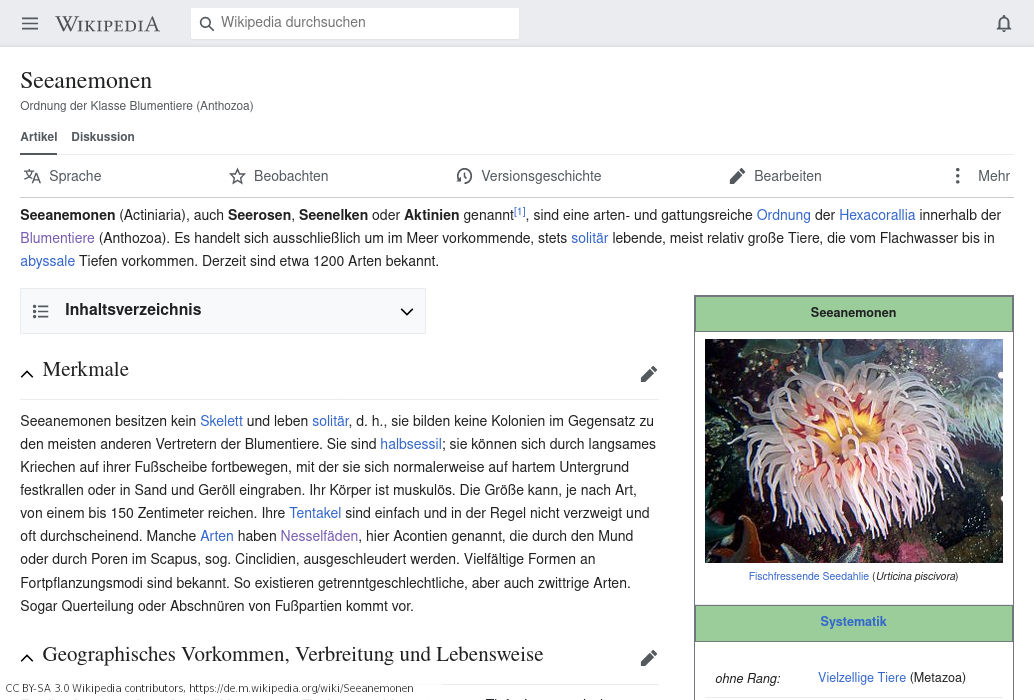
\includegraphics[height=0.75\textheight]{images/wikipedia-screenshot-2.jpg}};}
				\visible<4->{\node at (0.75, -0.75)	{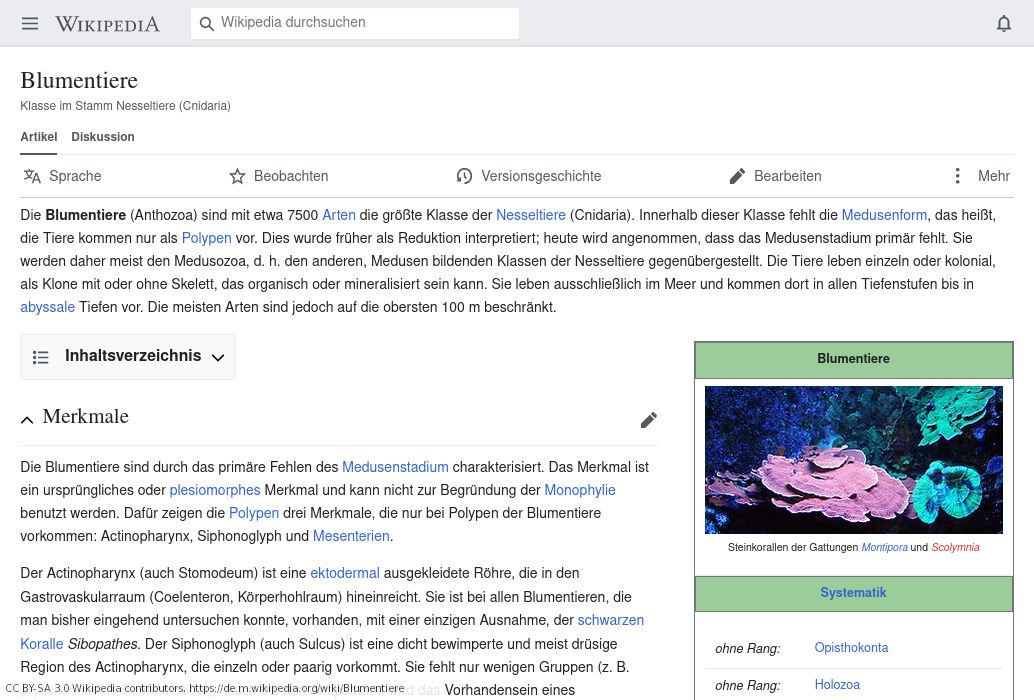
\includegraphics[height=0.75\textheight]{images/wikipedia-screenshot-3.jpg}};}
				\visible<5->{\node at (1, -1)		{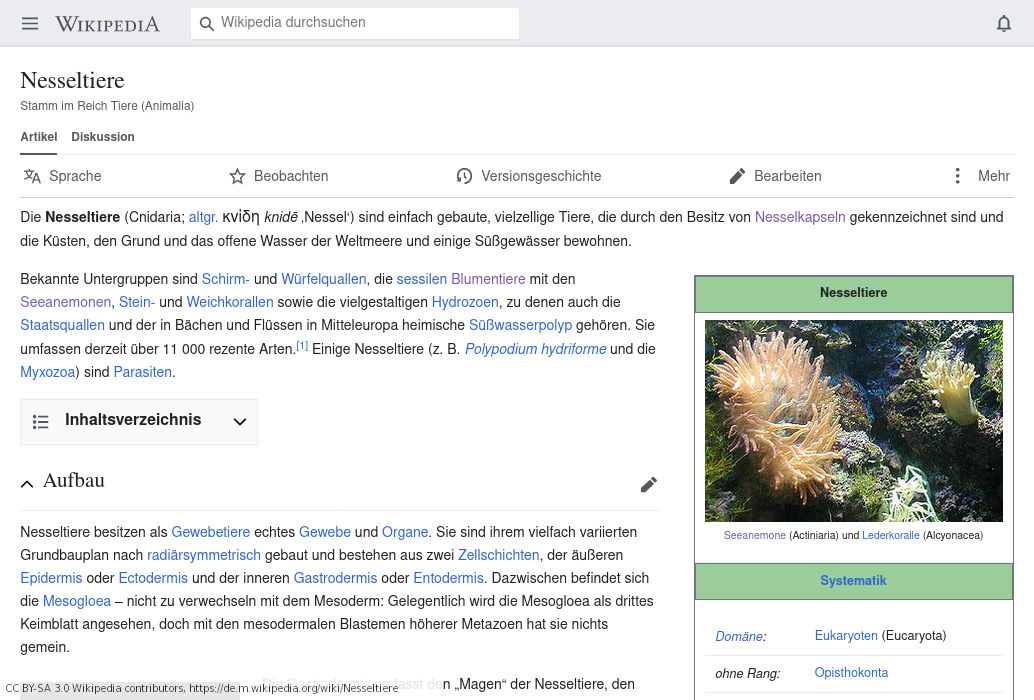
\includegraphics[height=0.75\textheight]{images/wikipedia-screenshot-4.jpg}};}
				\visible<6->{\node at (1.25, -1.25)	{
\includegraphics[height=0.75\textheight]{images/wikipedia-screenshot-5.jpg}};}
			\end{tikzpicture}
		\end{center}
	\end{frame}

	\begin{frame}
		\textit{"`Going on to Wikipedia to look something up, then unexpectedly being sucked into a seemingly \textbf{endless series of link clicking} to end up in a completely different part of wikipedia than you ever meant to go to."'}
		\n\hfill{\small--- \href{https://www.urbandictionary.com/define.php?term=Wikipedia\%20Hole}{Urban Dictionary}}
	\end{frame}

	\begin{frame}
		\begin{center}
			\only<1>{
\includegraphics[height=0.75\textheight]{images/meme-spongebob-gary-0.png}}
			\only<2>{
\includegraphics[height=0.75\textheight]{images/meme-spongebob-gary-1.png}}
		\end{center}
	\end{frame}

	\subsection{Existierende Tools}
	
	\begin{frame}
		\begin{itemize}
			\item \texttt{pandoc}
			\item \texttt{mediawiki2latex} / \texttt{wb2pdf}
			\item \texttt{epub-press}
			\item \texttt{w2eb}
			\item \texttt{percollate}
		\end{itemize}
	\end{frame}

	\begin{frame}{Warum gehen die nicht?}
		Inhaltliche \& visuelle Gründe:
		\begin{itemize}
			\item Formatierung, Schriftgrößen, etc. stimmt nicht
			\item Templates werden nicht/uneingeschränkt evaluiert
			\item \LaTeX/Math wird nicht in Bild gerendert
			\item Tabellen funktionieren nicht
		\end{itemize}
	\end{frame}

	\begin{frame}{Warum gehen die nicht?}
		Technische Gründe:
		\begin{itemize}
			\item Kann nicht mehrere Artikel gleichzeitig
			\item Bilder werden nicht heruntergeladen
			\item Wird nicht mehr maintained
			\item Ist in JavaScript
			\item Ist in einer Programmiersprache, die ich nicht kann / mag
			\item Ergebnis ist kein EPUB
			\item Ergebnis lief nicht auf meinem Tolino
		\end{itemize}
	\end{frame}
	
	% Was will ich haben? Was soll das Resultat sein?
	\subsection{Was will ich haben?}
	\begin{frame}
		\begin{center}
			\textbf{Generierte und gekaufte eBooks sollen sich qualitativ nicht unterscheiden.}
		\end{center}\pause
		Allgemeine Anforderungen:
		\begin{itemize}
			\item Formatierung stimmig
			\item Korrekte Übersetzung/Einbindung von Tabellen, Bilder, Listen, Quellenangaben, etc.
			\item Wikipedia-spezifische Templates \& Kategorien ignorieren
		\end{itemize}\pause\n
		Persönliche Anforderungen:
		\begin{itemize}
			\item Soll auf meinem Tolino eBook-Reader laufen
			\item Go als Programmiersprache
			\item Caching aller heruntergeladenen Daten (zum Coden im Zug)
		\end{itemize}
	\end{frame}

	\section{Wikipedia}	
	
	% Mediawiki Sprache
	\subsection{Wikitext -- Die Sprache der Wikipedia}
	
	\begin{frame}[fragile]{Formatierung}
		\begin{verbatim}
Wikitext ''kann'' auch '''Formattierung'''.

Und  '''sogar ''alles''' durcheinander'' geht.
		\end{verbatim}
		\hrule\n
		
\includegraphics[scale=0.35]{images/wikitext-example-0-formatting.png}
	\end{frame}
	
	\begin{frame}[fragile]{Links}
		\begin{verbatim}
Interne [[Hyperlink|Links]] gehen.

Auch ins Internetz [https://externe-links], sogar mit
[https://foo.bar Namen].
		\end{verbatim}
		\hrule\n
		
\includegraphics[scale=0.35]{images/wikitext-example-1-links.png}
	\end{frame}
	
	\begin{frame}[fragile]{Referenzen \& Templates}
		\begin{verbatim}
Hi<ref name="foo">{{Internetquelle|url=http://bar.de
|abruf=2022-10-12|titel=Ref mit Template}}</ref>!

Die selbe Ref. nochmal!<ref name="foo" />
		\end{verbatim}
		\hrule\n
		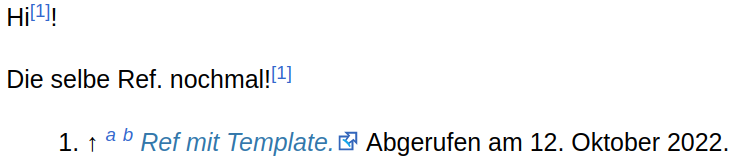
\includegraphics[scale=0.35]{images/wikitext-example-2-refs.png}
	\end{frame}
	
	\begin{frame}[fragile]{Überschriften}
		\begin{verbatim}
= Level 1 =
Wird nicht aktiv benutzt, da Titel der Seite h1 ist.

==== Level 4 ====
Die hier wird benutzt.
		\end{verbatim}
		\hrule\n
		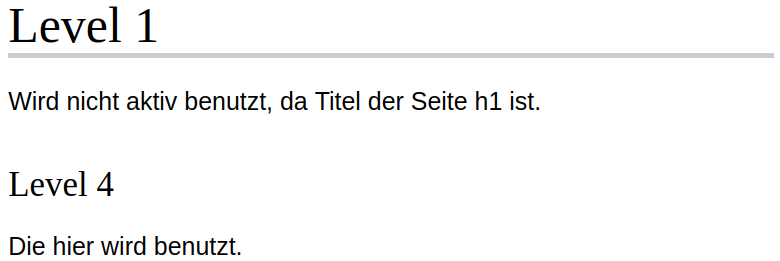
\includegraphics[scale=0.35]{images/wikitext-example-3-headings.png}
	\end{frame}

	\begin{frame}[fragile]{Listen}
		\begin{verbatim}
* Listen
** gibt
es
# auch
## noch
		\end{verbatim}
		\hrule\n
		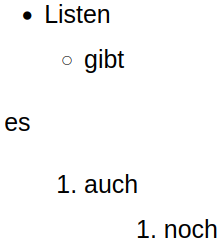
\includegraphics[scale=0.35]{images/wikitext-example-4-lists.png}
	\end{frame}

	\begin{frame}[fragile]{Tabellen}
		\footnotesize
		\begin{verbatim}
{| class="wikitable"
|-
! Spalte 1 !! Spalte 2
|-
| Hier
| könnte
|-
| ihre || Werbung stehen
|}
		\end{verbatim}
		\hrule\n
		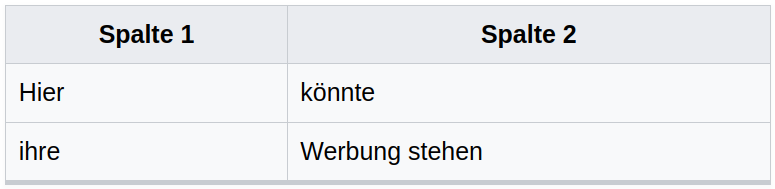
\includegraphics[scale=0.35]{images/wikitext-example-5-table.png}
	\end{frame}

	\begin{frame}[fragile]{Bilder}
		\begin{verbatim}
Hier ein Bild:

[[Datei:Full moon partially obscured by atmosphere.jpg
|mini|Mit Unterschrift.]]
		\end{verbatim}
		\hrule\n
		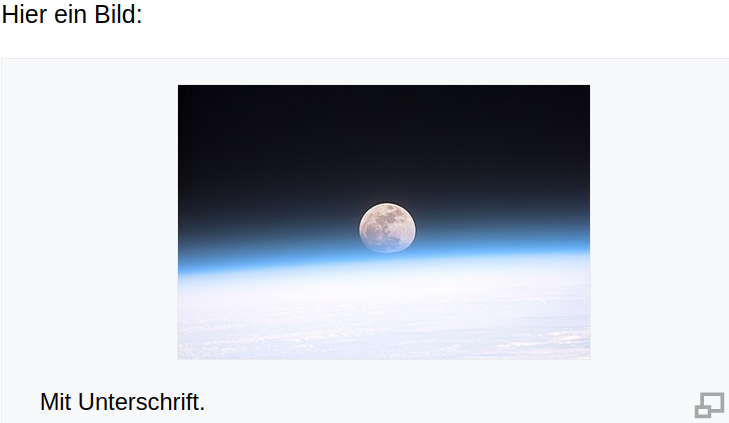
\includegraphics[scale=0.35]{images/wikitext-example-6-image.png}
	\end{frame}
	
	\begin{frame}{Und vieles mehr}
		\begin{itemize}
			\item Description list
			\item Zitate
			\item Einrückungen
			\item Code
			\item \LaTeX-Mathe-Zeug
			\item Musiknoten
			\item Gallerien
			\item Inline Bilder
			\item Diverse Parameter an allen möglichen Dingen
		\end{itemize}
	\end{frame}
	
	% Wie funktioniert Wikipedia?
	% - Aufbau (einzelne Instanzen, Wikimedia)
	% - Benötigte APIs und wie diese funktionieren
	\subsection{Instanzen \& APIs}
	
	\begin{frame}{Instanzen -- Artikel}
		\begin{itemize}
			\item Instanz pro Land/Sprache \textrightarrow\ z.B. [en\textbar de\textbar nds].wikipedia.org
			\item Verlinkungen ggf. zu anderen Instanzen möglich
		\end{itemize}
	\end{frame}

	\begin{frame}{Instanzen -- Bilder}
		\begin{itemize}
			\item Wikimedia commons (\href{https://commons.wikimedia.org}{commons.wikimedia.org})
			\item Normal:\newline \href{https://upload.wikimedia.org/wikipedia/commons/0/06/Foo.jpg}{upload.wikimedia.org/wikipedia/commons/0/06/Foo.jpg}
			\item Aber auch:\newline \href{https://upload.wikimedia.org/wikipedia/de/2/26/Son-3.jpg}{upload.wikimedia.org/wikipedia/\textbf{de}/2/26/Son-3.jpg}
			\pause
			
			\item Redirects möglich
			\begin{itemize}
				\item Beispiel: \href{https://commons.wikimedia.org/w/index.php?title=File:MET00506.jpg&action=edit}{\texttt{File:MET00506.jpg}}
				\item Ggf. ist Dateiname im Artikel $\neq$ Dateiname bei Wikimedia commons
				\item Nach Bild-Artikel suchen
				\item \texttt{redirects=true} Parameter nicht vergessen
			\end{itemize}
			\pause
			
			\item In Deutschen Artikeln wird natürlich \texttt{\textbf{Datei}:Sol-3.jpg} benutzt
		\end{itemize}
	\end{frame}

	\begin{frame}[fragile]{APIs -- Artikel abfragen}
		\textbf{Anfrage:}\\
		Puren Wikitext in JSON Antwort verpackt:\\
		\begin{verbatim}
GET  de.wikipedia.org/w/api.php
       ?action=parse
       &format=json
       &prop=wikitext
       &page={article name}
		\end{verbatim}\n
		\textbf{Antwort:}
		\begin{verbatim}
{
    "parse": {
        "title": "Erde",
        "wikitext": {
            "*": "..."
        }
    }
}
		\end{verbatim}
	\end{frame}

	\begin{frame}[fragile]{APIs -- Templates evaluieren}
		\textbf{Anfrage:}\\
		Wie bei Artikeln nur andere Parameter.\\
		\begin{verbatim}
GET  de.wikipedia.org/w/api.php
        ?action=expandtemplates
        &format=json
        &prop=wikitext
        &text={{mein tolles template}}
		\end{verbatim}\n
		\textbf{Antwort:}
		\begin{verbatim}
{
    "expandtemplates": {
        "wikitext": "..."
    }
}
		\end{verbatim}
	\end{frame}

	\begin{frame}{APIs -- Bilder}
		\textbf{Aufbau:}\\
		\texttt{upload.wikimedia.org/wikipedia/\{instance\}/}
		\texttt{\{MD5[0]\}/\{MD5[0]MD5[1]\}/\{filename\}}
		\n
		\textbf{MD5:}\\
		\texttt{MD5[i]} = Das \texttt{i}-te Zeichen des MD5-Hashes von \texttt{filename}
	\end{frame}

	\begin{frame}{APIs -- \LaTeX-Mathe in Bild umwandeln}
		\begin{enumerate}
			\item Math-check API für Resource location anfragen
			\item Eigentliches Bild abfragen
		\end{enumerate}
	\end{frame}

	\begin{frame}[fragile]{\LaTeX zu Bild: 1. Resource location bekommen}
		\textbf{Anfrage:}\\
		URL: \texttt{POST https://wikimedia.org/api/rest\_v1/media/math/check/tex}\\
		Body: URL encoded form Element \texttt{q} mit dem \LaTeX-Code:\n
		\verb+q:\sqrt{x}+
		\n
		\textbf{Antwort:}\\
		Header \texttt{x-resource-location} auslesen:\n
		\texttt{x-resource-location: 73b85c4ec364802ad746381712d10a43f073d50a}
	\end{frame}

	\begin{frame}[fragile]{\LaTeX zu Bild: 2. Bild abfragen}
		\textbf{Anfrage:}\\
		Einfaches \texttt{GET} mit Hash an\n
		\href{https://wikimedia.org/api/rest_v1/media/math/render/svg/73b85c4ec364802ad746381712d10a43f073d50a}{\texttt{wikimedia.org/api/rest\_v1/media/math/render/\{svg\textbar png\}/73b85c4...}}
	\end{frame}
		
	% Technische Strategie
	% - Umwandlung mediawiki -> HTML (weil EPUB HTML enthält) -> EPUB
	% - mediawiki -> HTML = Quasi Transpiler
	% - Wie funktioniert ein Compiler/Transpiler
	
	% Aufbau von wiki2book
	% - Einzelne Schritte:
	%  1. Clean
	%  2. Templates evaluieren
	%  3. Allerlei Dinge (Links, Bilder, Tabellen, Listen, ...)
	%  Solange zu 1 zurück springen bis alles fertig ist
	
	% Einzelheiten
	% - Parsen von Listen
	% - Parsen von Tabellen
	
	% Probleme, die aufgetreten sind
	
	% Infos (Repo, Bauen, CLI, ...)
	
	% Hands-on
\end{document}